\documentclass[../../relatorio.tex]{subfiles}

\begin{document}

\subsection{EMBI+ Brasil (Risco Brasil)}

\begin{figure}[ht]
  \begin{minipage}{0.70\textheight}
    \centering
      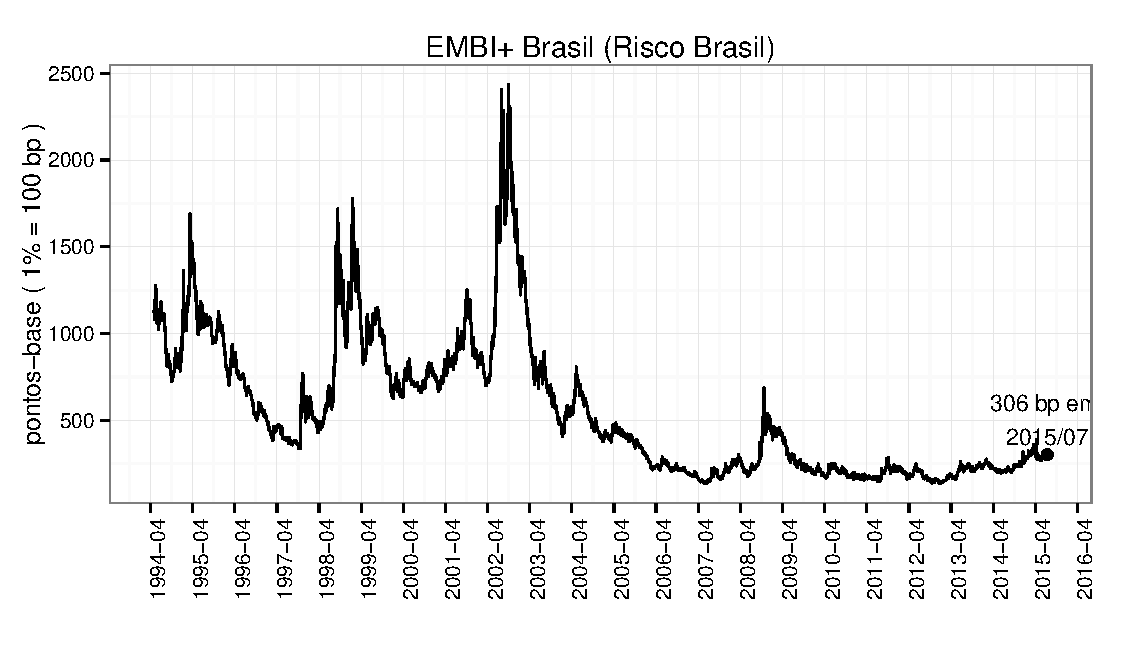
\includegraphics[width=17cm]{EMBI.pdf}
  \end{minipage}
\end{figure}

O risco-Brasil é um conceito que busca expressar de forma objetiva o risco de crédito a que investidores estrangeiros estão submetidos quando investem no País. No mercado, os indicadores diários mais utilizados para essa finalidade são o EMBI+Br e o Credit Default Swap (CDS) do Brasil.

O EMBI+Br é um índice que reflete o comportamento de títulos da dívida externa brasileira. A variação do índice entre duas datas permite calcular o retorno de uma carteira composta por esses títulos. O spread do EMBI+Br é o valor normalmente utilizado pelos investidores e público em geral como medida do risco Brasil e corresponde à média ponderada dos prêmios pagos por esses títulos em relação a papéis de prazo equivalente do Tesouro dos Estados Unidos, que são considerados livres de risco. Esse prêmio de risco é chamado no jargão mercado como spread over Treasury dessa carteira  Basicamente, o mercado usa o EMBI+Br para medir a capacidade do país honrar os seus compromissos financeiros , ou seja, quanto maior a pontuação do indicador de risco, maior é o risco de crédito do país a que se refere . Assim, para conseguir atrair capital estrangeiro em montante suficiente para o financiamento de sua dívida externa, um país com spread elevado no EMBI+ necessita oferecer altas taxas de juros em seus papéis. \footnote{http://www4.bcb.gov.br/pec/gci/port/focus/FAQ 9-Risco Pais.pdf}

\pagebreak
\end{document}
